\documentclass[10pt,twocolumn]{article}
\usepackage[a4paper,margin=1.5cm,bottom=1.45cm]{geometry}
\usepackage{titlesec}
\titlespacing*{\section}{0pt}{0.3em}{0.18em}
\usepackage[utf8]{inputenc}
\usepackage[T1]{fontenc}
\usepackage{lmodern}
\usepackage{graphicx}
\usepackage{booktabs}
\usepackage{microtype}
\usepackage[font=small,skip=4pt]{caption}
\usepackage[colorlinks=true,linkcolor=black,citecolor=black,urlcolor=blue]{hyperref}
\setlength{\columnsep}{0.7cm}

\title{\vspace{-0.9cm}\textbf{Budget-Aware Self-Configuring\\Neural Architecture Search for Unseen Data}\vspace{-0.15cm}}
\author{Sebastian Seifert, Luis Melzer \& Leander von Gottberg}
\date{\vspace{-0.65cm}}

\begin{document}
\maketitle

\section{Motivation}
The NAS Unseen-Data Challenge (AutoML 2026) evaluates a fully automated
pipeline on \emph{hidden} classification datasets under a strict
wall-clock budget per dataset. Inputs arrive as image-shaped tensors but
range from natural and satellite images to \emph{encoded} data (rendered
text, Sudoku boards, chess positions) where the spatial prior of a CNN
misleads. All decisions must be made at runtime, blind.

Our starting point is the winning method of the 2025 edition, EGNAS
\cite{egnas}, a macro--micro search (depth, width, per-layer operation)
over convolutional blocks. Reproducing it surfaced two
weaknesses. First, rankings from short training runs are unreliable:
operations that lead early often lose after full training, so fine-grained
(micro) operation search tends to \emph{harm} final accuracy. Second, the
space is confined to one family: in our experiments a \emph{fixed} 2-D
dilated-convolution backbone (temporal convolutional networks \cite{tcn})
beat the fully searched CNN on most datasets, while plain CNNs and random
architectures won on the encoded ones, matching random search as a strong
NAS baseline \cite{geada,li2019}. The leverage is choosing the right
architecture \emph{family} per dataset, not operation search.

\section{Research Questions}
\textbf{RQ1.} Can macro--micro NAS \cite{egnas} be generalised across
heterogeneous architecture families (plain CNNs, 2-D dilated and 1-D
temporal convolution networks), making families \emph{comparable} within a
single time-budgeted search stage despite the known unreliability of
low-fidelity rankings \cite{white2021}?
\textbf{RQ2.} Can cheap, training-free measurements of the raw data decide
at runtime which architectural prior fits an unseen dataset?
\textbf{RQ3.} How can harmful data augmentation be detected at runtime,
given that augmentation acts as regularisation (it costs accuracy early
and pays late) and that, as we observe, its decisions do not transfer
between architecture families?

\section{Approach}
We propose a self-configuring pipeline that measures the data first,
gates every decision, and spends all remaining time on training
(Fig.~\ref{fig:pipe}, p.~2). At its core is one search principle applied
at every level: each choice is searched against a robust incumbent
default, scored by a short-training proxy, and adopted only when it beats
the default beyond the proxy noise \emph{and} survives a longer
verification re-training. The search is reliability-aware by design, never
trusting a short-training ranking alone, the failure mode that makes naive
operation search harmful.
(1)~\emph{Measure}: a fingerprint computed directly from the raw input
tensors, with no training involved. The mean correlation of neighbouring
pixels separates the two data families with a wide margin: between
$-0.05$ and $0.07$ on the four encoded public datasets versus $0.38$ to
$1.00$ on all others. (2)~\emph{Family selection}: image-like data goes to the dilated
backbone directly; encoded data, where the prior is ambiguous, evaluates
all families at matched wall-clock and adopts the leader only when it
clears the default beyond the ranking noise, otherwise \emph{abstaining}
to the default (a built-in null hypothesis that bounds the downside).
(3)~\emph{Augmentation probe}: a two-arm test run \emph{after} the family
choice, with arms of the chosen family; it deviates only on a clear
margin (RQ3).
(4)~\emph{Structural search}: depth and width are searched against an
incumbent default, adopting a non-default choice only when it wins beyond
the proxy noise \emph{and} survives re-training verification at a longer
horizon. (5)~\emph{Operation-level exploration}: on encoded data with
budget to spare, the search samples architectures from a broad operation
vocabulary under the same verify-before-adopt rule; random sampling is a
deliberate, competitive NAS baseline \cite{li2019}. (6)~\emph{Train to budget}: the winner trains on
the full remaining time with a cosine learning-rate schedule \cite{sgdr}
sized to reach zero exactly when the budget ends. All stage budgets are
fractions of the clock, so the pipeline degrades gracefully from many
hours down to minutes.





\section{Required Steps}
(1)~Reproduce the EGNAS baseline and probe candidate architecture
families at full budget (done). (2)~Validate each decision mechanism in
isolation against known full-budget outcomes. (3)~Integrate the pipeline
and verify all execution paths, including low-budget collapse.
(4)~Full multi-seed evaluation. (5)~A budget-ladder study (0.5h to 8h)
measuring which stages pay at which budget. (6)~A generalisation test on
untouched external datasets. (7)~Packaging and stress tests.

\section{Evaluation Strategy}
Primary evaluation uses the 13 public competition datasets with the
official adjusted score (accuracy versus a per-dataset benchmark, capped),
at least three seeds for final configurations. Baselines: the reproduced
EGNAS search, each fixed family, and a best-family oracle bounding the
achievable routing gain. Every stage writes its measurements, margins,
and choices to a per-dataset decision record, so gains and losses are
attributable to individual decisions. Robustness is evaluated across
budgets (30 minutes to 12 hours), on the external suite, and against
published competition bests \cite{geada}. First results of the current pipeline, including the
configuration it selects per dataset, are shown in
Fig.~\ref{fig:res} (p.~3).

\section{Potential Extensions}
The pipeline scales with the budget: at large budgets it admits extra
families (recurrent and attention blocks) via the gated comparison and
searches per-stage \emph{heterogeneous} architectures rather than one
uniform stack; on ties it trains a cross-family ensemble, kept only if it
beats the best single model. We also build competition-style datasets
blind to the pipeline as a generalisation test.



\clearpage
\onecolumn
\begin{figure}[p]
\centering
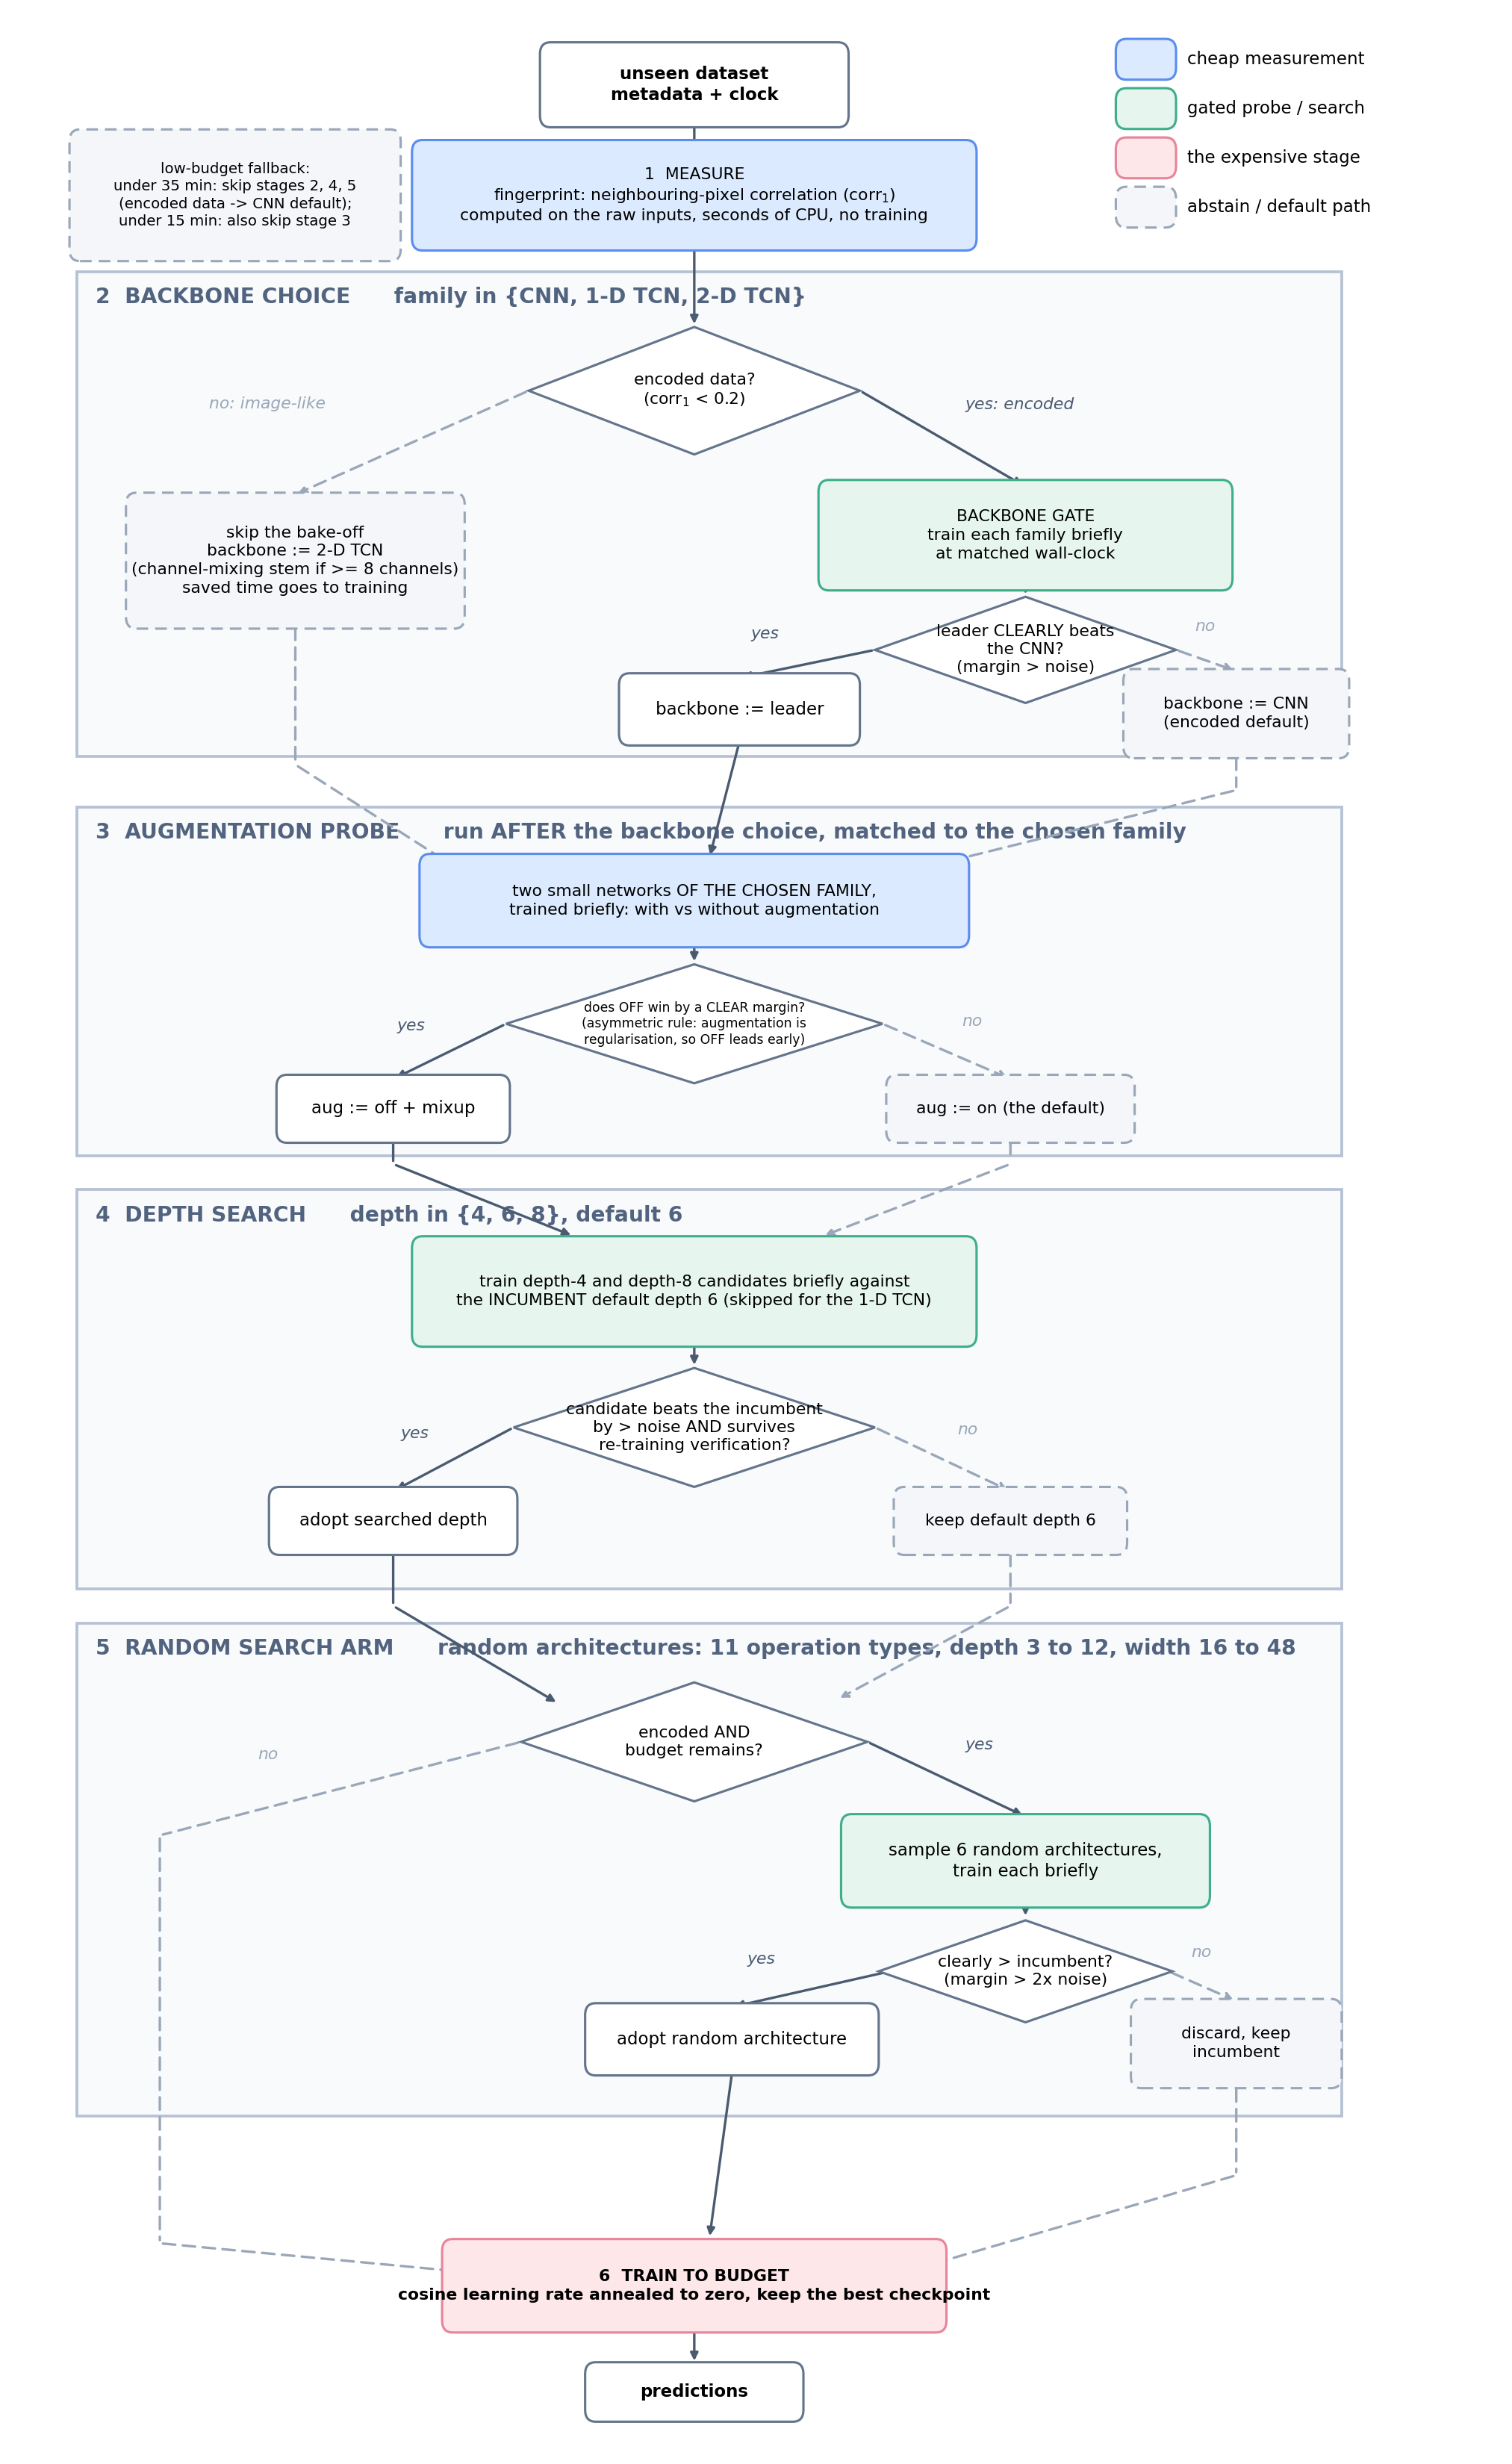
\includegraphics[width=\textwidth,height=0.92\textheight,keepaspectratio]{pipeline.png}
\caption{The decision pipeline, run once per unseen dataset. Diamonds
are runtime decisions, dashed paths are the abstain-to-default routes.}
\label{fig:pipe}
\end{figure}

\clearpage
\begin{figure}[p]
\centering
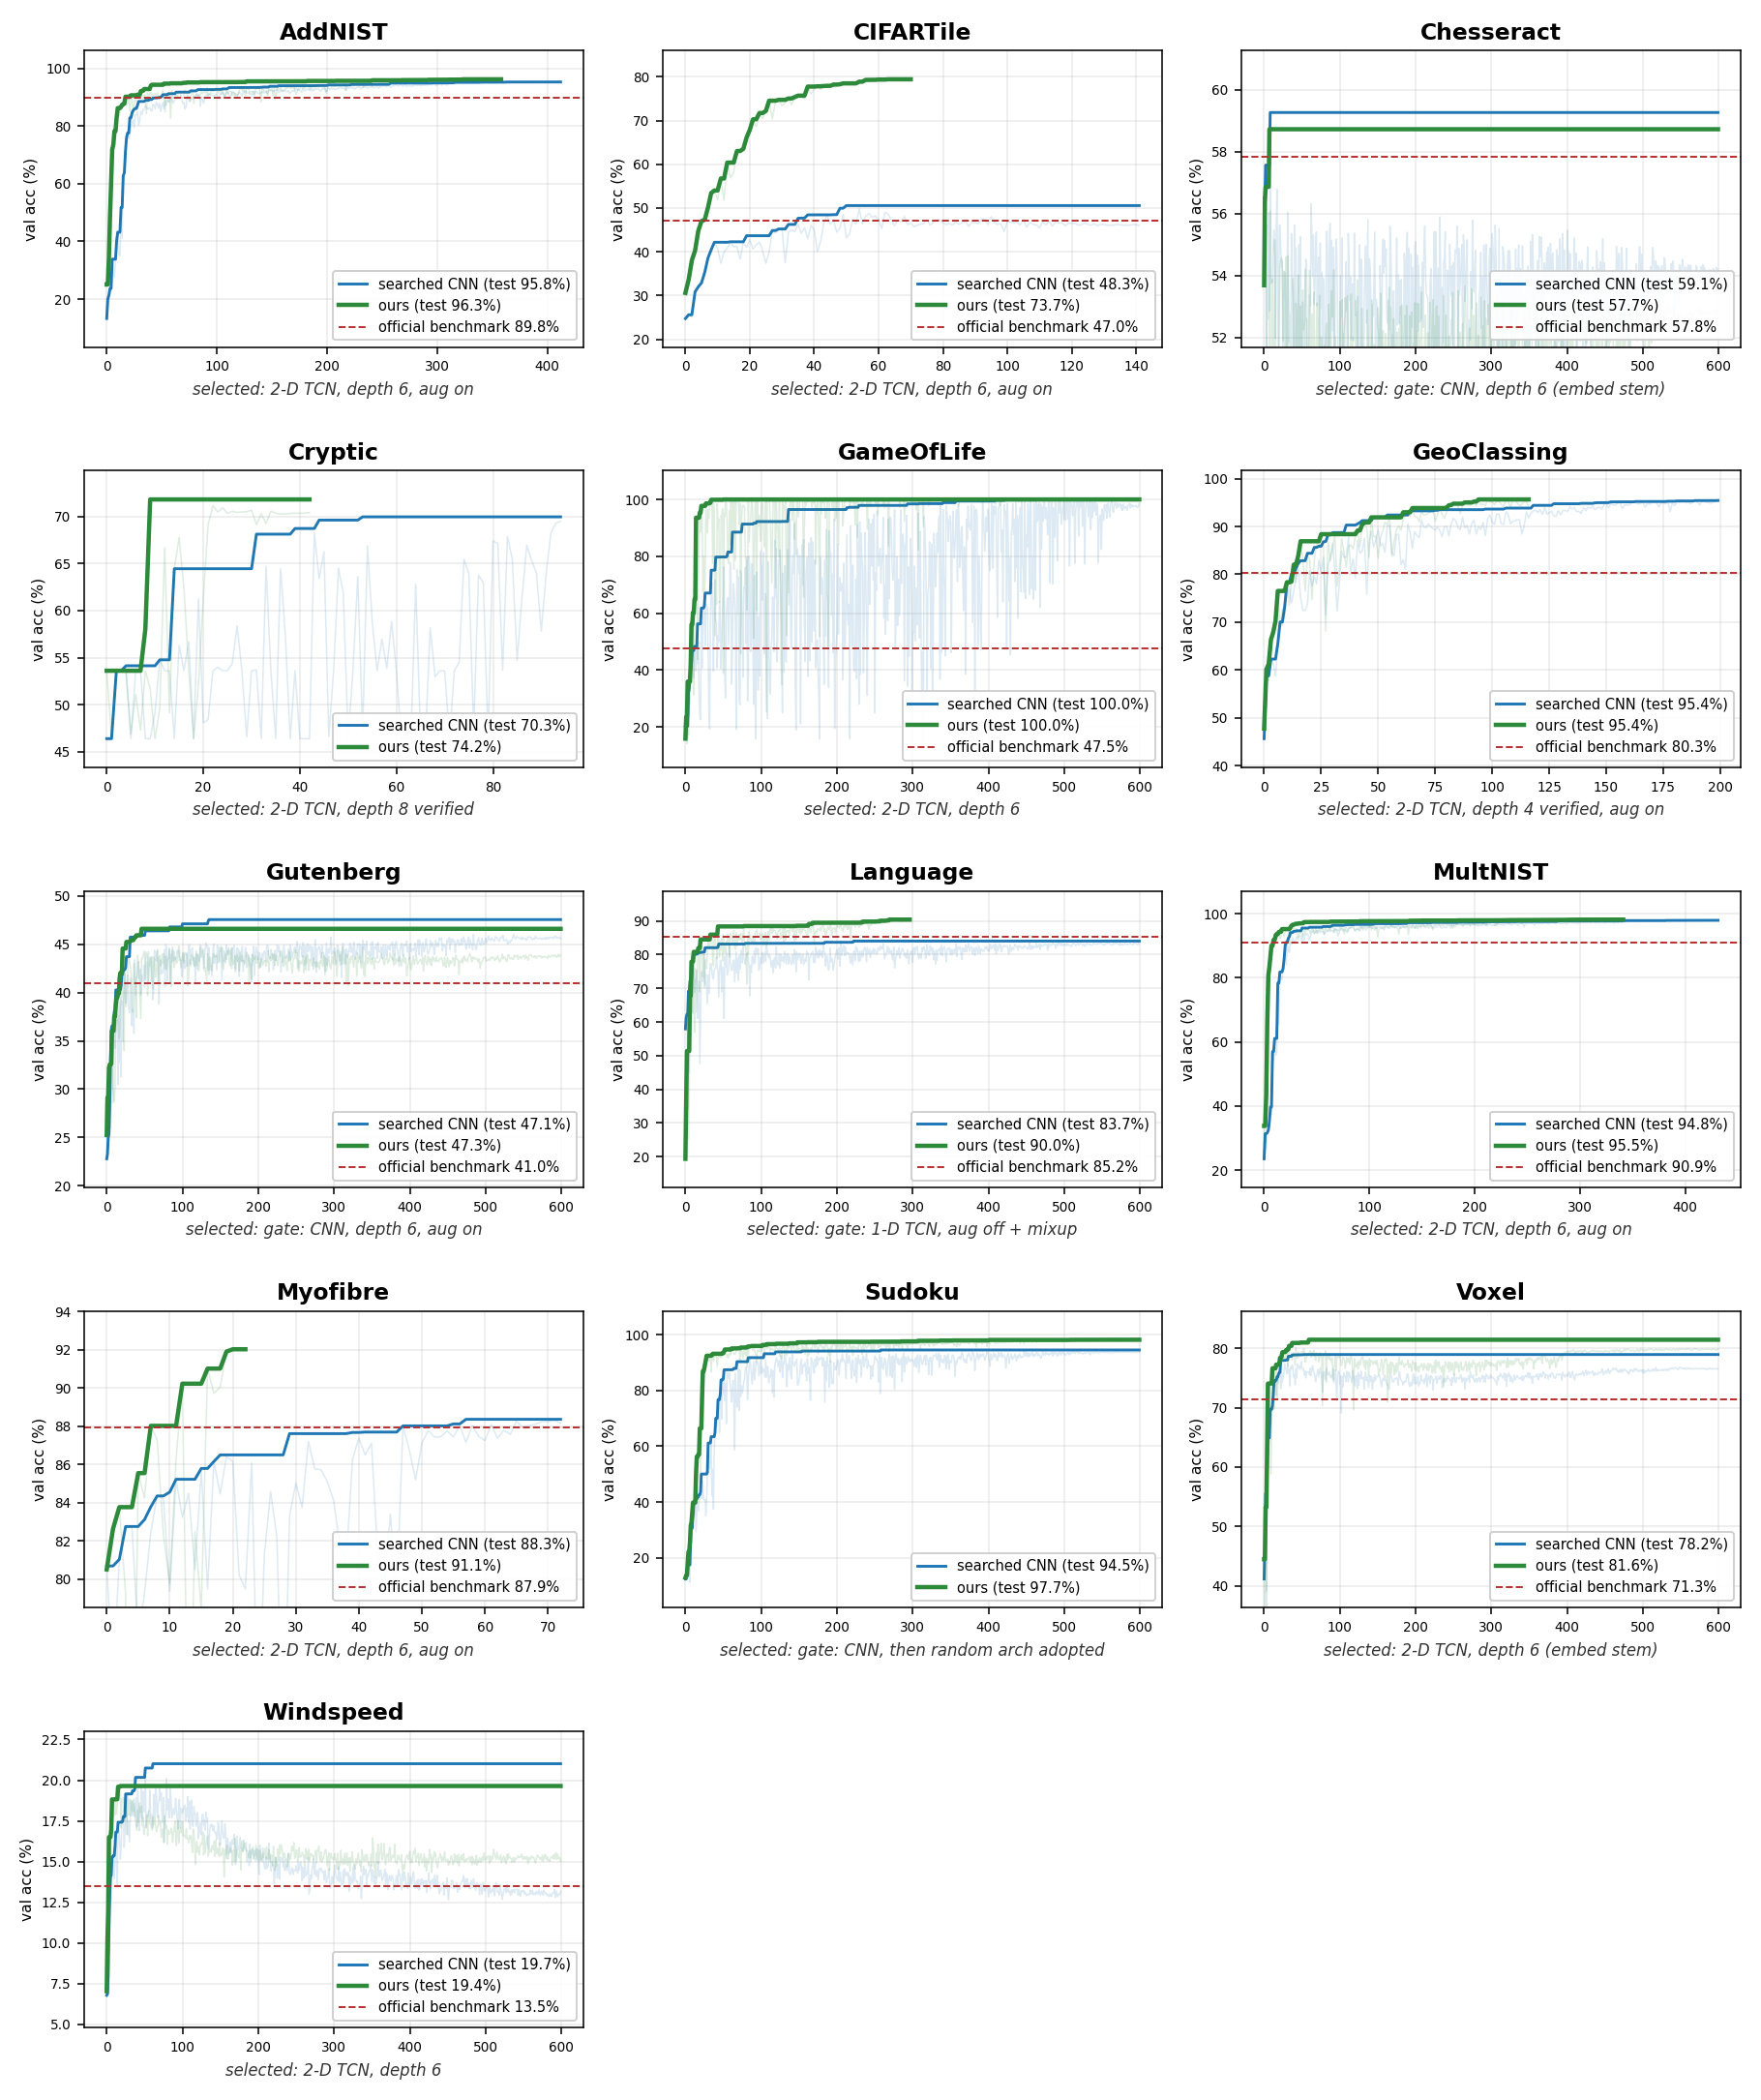
\includegraphics[width=\textwidth,height=0.85\textheight,keepaspectratio]{results_grid.png}
\caption{Our current best approach versus the searched CNN (our reproduction of
the winning macro--micro NAS \cite{egnas} with identical training
improvements), 13 public datasets, single seed, 2~h per dataset on a
single GB10. Curves:
validation accuracy (faint per-epoch, solid best-so-far). Legends: final
test accuracy, which can differ from validation. Red dashed: the
official benchmark from the dataset metadata; unpublished for Sudoku and
Cryptic. The selected configuration is noted under each panel. Totals
(adjusted score): ours \textbf{+62.5}, searched CNN +48.2.}
\label{fig:res}
\end{figure}

\clearpage
\begin{thebibliography}{9}\footnotesize\setlength{\itemsep}{1pt}\setlength{\parskip}{0pt}
\bibitem{egnas} S.~Siddiqui, C.~Kyrkou, T.~Theocharides.
\emph{Efficient Global Neural Architecture Search}. SN Computer Science
6:282, 2025.
\bibitem{geada} R.~Geada, D.~Towers, M.~Forshaw, A.~Atapour-Abarghouei,
A.~S.~McGough. \emph{Insights from the Use of Previously Unseen Neural
Architecture Search Datasets}. CVPR 2024.
\bibitem{tcn} S.~Bai, J.~Z.~Kolter, V.~Koltun. \emph{An Empirical
Evaluation of Generic Convolutional and Recurrent Networks for Sequence
Modeling}. arXiv:1803.01271, 2018.
\bibitem{li2019} L.~Li, A.~Talwalkar. \emph{Random Search and
Reproducibility for Neural Architecture Search}. UAI 2019.
\bibitem{white2021} C.~White, A.~Zela, B.~Ru, Y.~Liu, F.~Hutter.
\emph{How Powerful are Performance Predictors in Neural Architecture
Search?} NeurIPS 2021.
\bibitem{sgdr} I.~Loshchilov, F.~Hutter. \emph{SGDR: Stochastic Gradient
Descent with Warm Restarts}. ICLR 2017.
\end{thebibliography}

\end{document}
